\documentclass[11pt]{beamer}
\usetheme{Malmoe}
\usepackage[utf8]{inputenc}
\usepackage{amsmath}
\usepackage{amsfonts}
\usepackage{amssymb}
\usepackage{tikz}
\usepackage{graphicx}
\usepackage{listings}
\usepackage{color}

\author{zach wick \\ zwick@bareo.io}
\title{Making Sense of CORS using web.py}

\begin{document}

\lstset{
  keywordstyle=\color{blue},
  showspaces=false,
  showstringspaces=false,
  basicstyle=\tiny
}

\begin{frame}
  \titlepage
\end{frame}

\begin{frame}{Agenda}
  \begin{itemize}
  \item About the speaker\\
  \item HTTP Primer\\
  \item What is CORS\\
  \item Why is CORS useful\\
  \item How does CORS work\\
    \begin{itemize}
    \item HTTP\\
    \item Simple Requests\\
    \item Other Requests\\
    \end{itemize}
  \item Worked Example\\
  \item Best Practices\\
  \item Questions (and hopefully answers)
  \end{itemize}
\end{frame}

\begin{frame}{About the Speaker}
 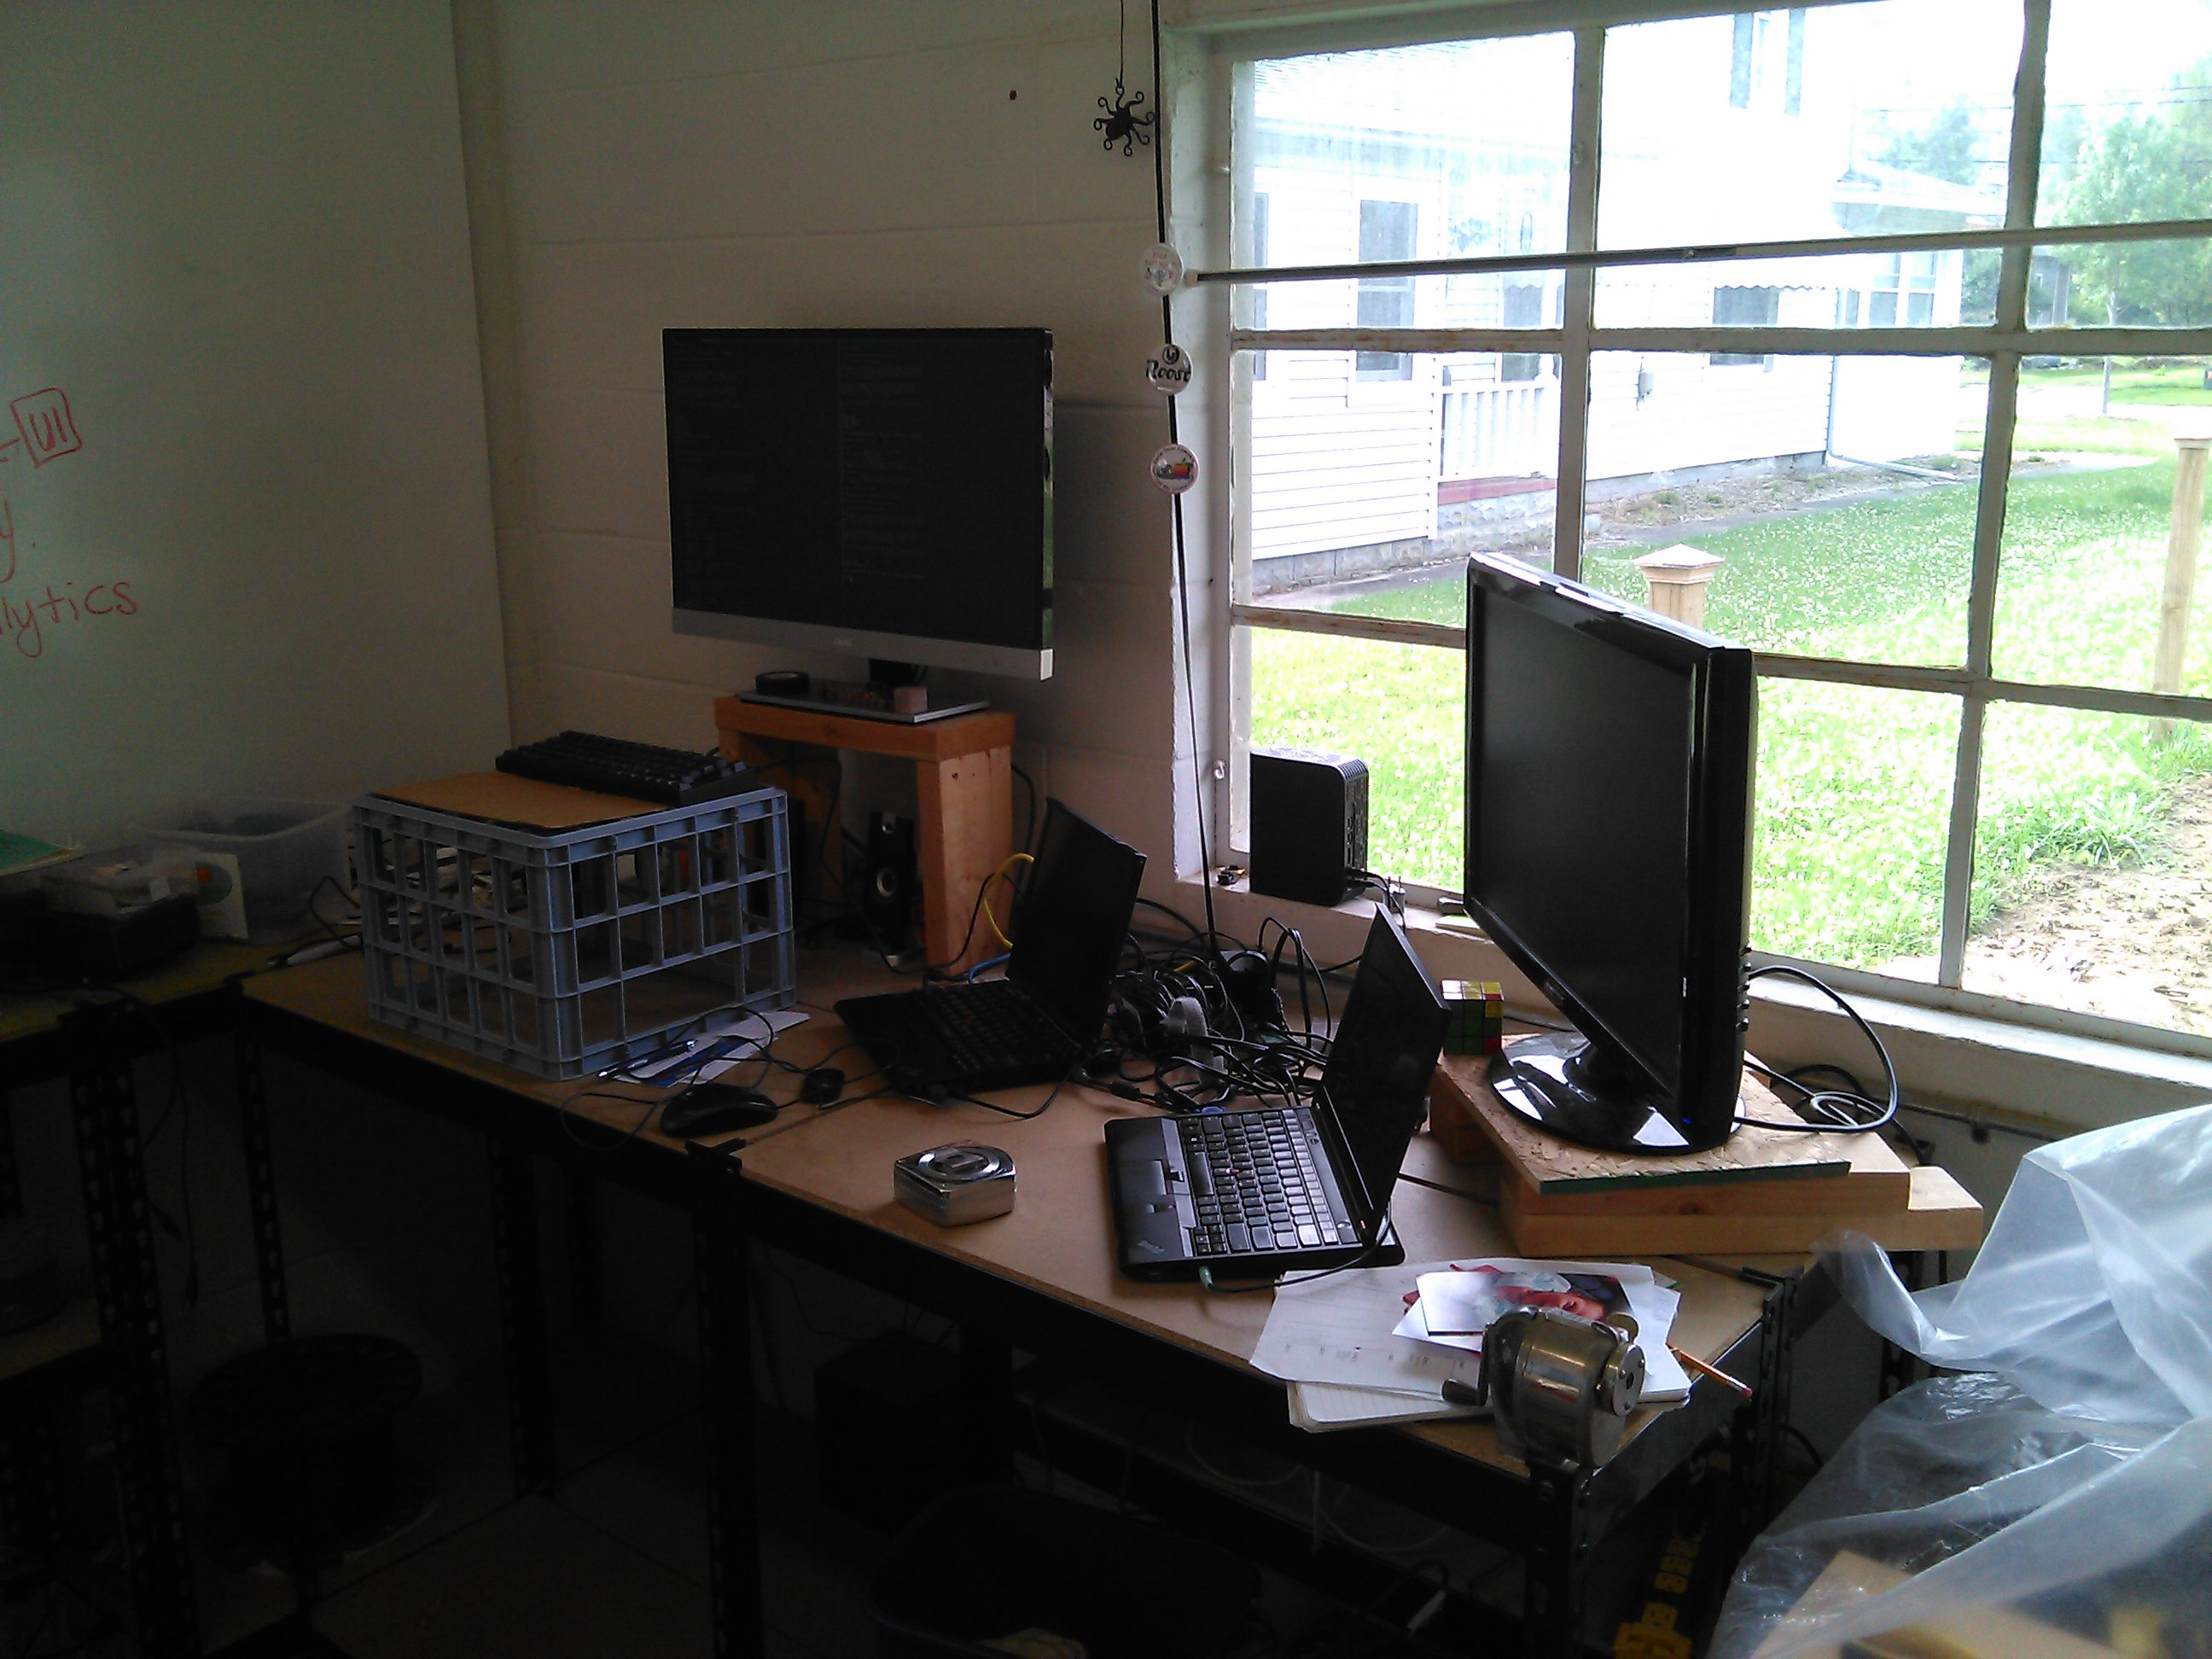
\includegraphics[keepaspectratio=true,width=\framewidth]{shop.jpg}
\end{frame}

\begin{frame}{HTTP Primer}
  \begin{itemize}
  \item application protocol\pause
  \item uses request verbs\pause
    \begin{itemize}
    \item HTTP/1.0 | GET POST HEAD\pause
    \item HTTP/1.1 | OPTIONS PUT DELETE TRACE CONNECT\pause
    \item RFC 5789 | PATCH\pause
    \item Other specs \& RFC's\pause
    \item * Other user defined verbs *\pause
    \end{itemize}
  \item idempotent vs. non-idempotent\pause
  \item status codes
  \end{itemize}
\end{frame}

\begin{frame}
  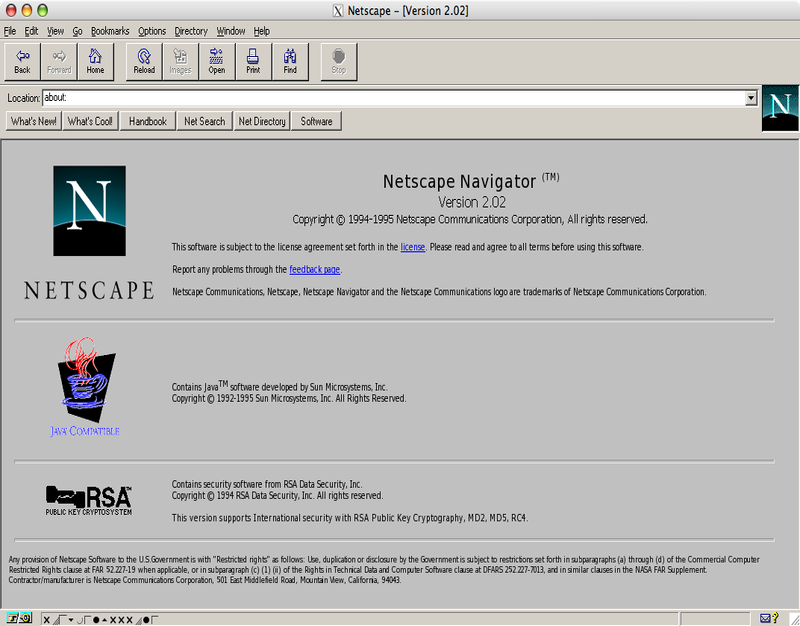
\includegraphics[keepaspectratio=true,width=\framewidth]{netscapenavigator2.png}
\end{frame}

\begin{frame}{In the Beginning There Was Netscape Navigator 2}
  \begin{itemize}
  \item LiveScript (now called JavaScript)\pause
  \item Plugin Support\pause
  \item HTML Frames (iframes)\pause
  \item Same-Origin Policy
  \end{itemize}
\end{frame}

\begin{frame}{Same-Origin Policy}
  \begin{itemize}
  \item Applies to DOM manipulation and others (XMLHttpRequest)\pause
  \item (protocol, host, port) = Origin\pause
  \item Tuples must match\pause
  \end{itemize}
  http://www.example.com/dir/page.html\pause\\
  \begin{tabular}{|l|c|l|}
    \hline
    Compared URL & Reason\\
    \hline
    http://www.example.com/dir/p2.html\pause & Origin Tuple Matches\\
    http://www.example.com/d2/p3.html\pause & Origin Tuple Matches\\
    https://www.example.com/dir/p2.html\pause & Protocol Differs\\
    http://www.example.com:82/dir/p2.html\pause & Port Differs\\
    http://example.com/dir/p2.html\pause & Host Differs\\
    http://www.example.com:80/dir/p2.html\pause & Implementation Based\\
    \hline
  \end{tabular}
\end{frame}

\begin{frame}{How to Get Around Same-Origin Policy}
  
\includegraphics[keepaspectratio=true,width=\framewidth]{circumvent.jpeg}
\end{frame}

\begin{frame}{What Do We Want?}
  \begin{columns}[t]
    \begin{column}[t]{5cm}
      \textbf{Any Domain}\pause
      \hline
      \begin{itemize}
      \item images\pause
      \item scripts\pause
      \item stylesheets\pause
      \item iframes\pause
      \item videos\pause
      \item some plugin content\pause
      \end{itemize}
    \end{column}
    \begin{column}[t]{5cm}
      \textbf{Only Special Domains}\pause
      \hline
      \begin{itemize}
      \item embedded web fonts\pause
      \item AJAX
      \end{itemize}
    \end{column}
  \end{columns}
\end{frame}

\begin{frame}{What about JSONP?}
  \begin{itemize}
  \item JSON with padding\pause
  \item works via HTML script tags (in the 'Any Domain' column)\pause
  \item only GET
  \end{itemize}
\end{frame}

\begin{frame}{Why is CORS useful?}
  \begin{itemize}
    \item AJAX to non-origin domains
  \end{itemize}
\end{frame}

\begin{frame}{How does CORS work?}

\end{frame}

\end{document}
